% arXiv submission bundle -- generated from ../main.tex, figure paths flattened to figs/
% Regenerate with the sync step in SUBMISSION.md; do not hand-edit.
% Preprint: conjunctival pallor screening on CP-AnemiC
% Build: tectonic main.tex
% Figures are read from ../results/, regenerated by scripts/run_full_analysis.py
%         and scripts/make_extra_figures.py
\documentclass[11pt,a4paper]{article}

\usepackage[margin=2.5cm]{geometry}
\usepackage[T1]{fontenc}
\usepackage{lmodern}
\usepackage{microtype}
\usepackage{amsmath,amssymb}
\usepackage{booktabs}
\usepackage{graphicx}
\usepackage{caption}
\usepackage{siunitx}
\usepackage[hidelinks]{hyperref}
\usepackage{xcolor}
\usepackage{authblk}
\usepackage{abstract}

\captionsetup{font=small,labelfont=bf}
\sisetup{detect-weight=true}

\newcommand{\gdl}{\ensuremath{\mathrm{g/dL}}}
\newcommand{\auroc}{AUROC}

\title{\bfseries Duplicate leakage in a public conjunctival pallor benchmark,\\
and an honest baseline for image-based anaemia screening}

\author[1]{Paing Hein Htet}
\affil[1]{Department of Medical Physics and Biomedical Engineering,
University College London, London, United Kingdom}
\affil[ ]{\texttt{zcemphh@ucl.ac.uk}}
\date{\today}

\begin{document}
\maketitle

\begin{abstract}
\noindent
Conjunctival pallor photographs are an attractive substrate for non-invasive anaemia
screening, and CP-AnemiC --- 710 images of Ghanaian children aged 6--59 months with paired
laboratory haemoglobin --- has become a convenient public benchmark for the task. We report
that the benchmark contains duplicate records substantial enough to change published
conclusions, and we provide a corrected baseline.

Of the 710 metadata rows only 479 are distinct photographs: 212 files are byte-identical
copies registered under different image identifiers, and a further 19 are pixel-identical
after region-of-interest extraction while differing at the byte level, so content hashing
alone does not detect them. Ninety duplicate groups carry \emph{conflicting} haemoglobin
labels on identical pixels, one spanning 3.3 to 10.4~\gdl. Evaluating with a random split
therefore trains and tests on the same photograph and inflates \auroc{} by
$+0.103$ (95\,\% CI $+0.056$ to $+0.152$; bootstrap $p<0.001$, $n_{\text{boot}}=5000$).

After removing this redundancy and grouping cross-validation by collection site, twelve
interpretable colour features reach \auroc{} $0.780$ (95\,\% CI $0.737$--$0.818$) for WHO
anaemia ($\mathrm{Hb}<11$~\gdl), against a demographics-only floor of $0.565$; the image
contributes $+0.215$ \auroc{} (DeLong 95\,\% CI $+0.151$ to $+0.279$,
$p=4.4\times10^{-11}$). Bland--Altman limits of agreement nonetheless span
$7.3$~\gdl{} with strong proportional bias (slope $-0.67$), so the model is a triage
screen and not a haemoglobin meter. At a threshold catching 90\,\% of anaemic children,
specificity falls to $0.362$, and decision curve analysis shows the model is worse than
referring every child below a threshold probability of about $0.15$ --- so it earns
its place only where confirmatory testing is scarce.

We recommend that future work on CP-AnemiC deduplicate at the pixel level and group
cross-validation by site, and we release the full analysis so that reported numbers can be
checked against these controls.
\end{abstract}

\medskip
\noindent\textbf{Keywords:} anaemia screening; conjunctival pallor; data leakage;
benchmark integrity; medical imaging; low-resource diagnostics.

\section{Introduction}

Anaemia affects an estimated 40\,\% of children aged 6--59 months worldwide, rising to
68\,\% in west and central Africa~\cite{stevens2022}, and diagnosis
conventionally requires a blood draw and laboratory or point-of-care haemoglobin assay.
Both are constrained in low-resource settings by cost, consumables, trained staff and
infection-control requirements. This has motivated interest in image-based screening: the
palpebral conjunctiva is a mucous membrane whose colour is visibly influenced by
haemoglobin concentration, is straightforward to expose, and can be photographed with a
consumer smartphone.

Public datasets are what allow such methods to be compared. CP-AnemiC
\cite{asare2023cpanemic} pairs conjunctiva photographs of Ghanaian children with laboratory
haemoglobin and has been adopted as a benchmark for this task. The value of any benchmark,
however, rests on an assumption that is rarely re-examined once a dataset is in circulation:
that its records are distinct. Where they are not, a randomly partitioned evaluation places
copies of the same photograph in both training and test folds, and the resulting score
measures memorisation rather than generalisation.

This paper makes three contributions.

\begin{enumerate}
  \item We show that CP-AnemiC contains duplicate records at a scale that materially
        inflates reported performance, and we quantify that inflation.
  \item We establish a corrected baseline under pixel-level deduplication and
        site-grouped cross-validation, using interpretable colour features only.
  \item We characterise the resulting model as a screening instrument --- reporting the
        operating point, calibration and Bland--Altman agreement that determine whether it
        could be deployed --- and conclude that it is not yet adequate as a haemoglobin
        estimator.
\end{enumerate}

Our aim is deliberately not a new architecture. It is to establish what the honest number
on this benchmark is, and to make the controls that produce it reproducible.

\section{Data}

\subsection{Source}

CP-AnemiC \cite{asare2023cpanemic} comprises conjunctiva photographs of children aged
6--59 months collected at ten hospitals across four Ghanaian regions, each paired with a
laboratory haemoglobin measurement. We use the WHO threshold for childhood anaemia,
$\mathrm{Hb}<11$~\gdl~\cite{who2011}. Table~\ref{tab:data} summarises the dataset as distributed and after
the deduplication described below.

\begin{table}[htbp]
\centering
\caption{CP-AnemiC as distributed and after deduplication.}
\label{tab:data}
\small
\begin{tabular}{lr}
\toprule
Property & Value \\
\midrule
Metadata rows (as distributed)      & 710 \\
Distinct images by SHA-256          & 498 \\
\textbf{Distinct images at pixel level} & \textbf{479} \\
Rows appearing exactly once         & 407 \\
Duplicate groups with conflicting Hb & 90 \\
Collection sites                    & 10 hospitals, 4 regions \\
Cohort                              & children 6--59 months \\
Label                               & laboratory Hb (\gdl); WHO threshold 11 \\
Anaemia prevalence after dedup      & 0.493 \\
\bottomrule
\end{tabular}
\end{table}

\subsection{Duplicate structure}

Two distinct forms of redundancy are present. \emph{Byte-identical} duplication accounts for
212 files: the same image registered under more than one identifier, detectable by hashing
the file. A further 19 images are \emph{pixel-identical after region-of-interest extraction}
but differ at the byte level --- re-encoded or re-saved copies --- and are therefore invisible
to content hashing. Detecting these requires comparing decoded pixels within the annotated
region, which is how the count falls from 498 to 479.

The consequential subset is the 90 duplicate groups carrying conflicting haemoglobin labels
on identical pixels. One such group spans 3.3 to 10.4~\gdl. Because the pixels are the same,
no model can satisfy both labels; the disagreement is irreducible label noise that places a
ceiling on achievable performance. Where duplicates were merged we took the median
haemoglobin, which is a defensible summary but cannot recover the truth.

\subsection{Mask handling}

Each image is RGBA, where the alpha channel is a hand-drawn conjunctiva mask covering
approximately 25\,\% of the frame; the remainder is black padding. Colour statistics must
therefore be computed over masked pixels only. Ignoring the mask shifts mean RGB by more
than $100/255$ and produces features that encode \emph{mask area} --- an artefact of
annotator behaviour --- rather than tissue colour.

\section{Methods}

\subsection{Features}

We extract twelve interpretable colour features over the masked region of interest: mean
$R$, $G$, $B$; circular mean hue and hue concentration; mean saturation; CIELAB $L^*$,
$a^*$, $b^*$; an illumination-normalised redness index $r/(r+g+b)$; its 10th percentile; and
the red/green ratio. The $a^*$ channel is the perceptual red--green axis that corresponds to
what a clinician reads as pallor.

Two exclusions are deliberate. \textbf{Mask area is not used as a feature}: it reflects how
the annotator drew the boundary rather than physiology, and had it correlated with site or
severity the model would have learned the annotator. \textbf{Hue is averaged circularly}:
red tissue sits near both $0.0$ and $1.0$ on the hue circle, so a linear mean of $0.98$ and
$0.02$ returns $0.5$, which is cyan.

\subsection{Model and validation}

A gradient-boosted regressor predicts haemoglobin; negating its output yields a screening
score. Hyperparameters were fixed \emph{a priori} and never tuned on this data; a nested
cross-validation check (Section~\ref{sec:controls}) confirms this cost essentially nothing.
All reported metrics are out-of-fold.

The validation protocol combines two requirements. Deduplication must operate at the pixel
level, for the reasons above. Cross-validation folds must be grouped by collection site, so
that a model cannot exploit site-specific camera, lighting or operator signatures shared
between training and test folds. We report a waterfall over both.

\section{Results}

\subsection{Progressive removal of optimism}

Table~\ref{tab:waterfall} evaluates the same colour features under successively stricter
protocols. Each row closes one more leak than the row above.

\begin{table}[htbp]
\centering
\caption{Effect of evaluation protocol on apparent performance. Colour features only.}
\label{tab:waterfall}
\small
\begin{tabular}{lrcc}
\toprule
Configuration & $n$ & \auroc{} [95\,\% CI] & MAE (\gdl) \\
\midrule
Random split, duplicates kept \emph{(common setup)} & 710 & 0.883 [0.858--0.906] & 1.46 \\
Exact duplicates removed, random split              & 498 & 0.796 [0.758--0.834] & 1.44 \\
\quad + grouped by collection site                  & 498 & 0.809 [0.772--0.847] & 1.42 \\
\textbf{\quad + pixel-level duplicates removed (headline)}
                                                    & \textbf{479}
                                                    & \textbf{0.780 [0.737--0.818]}
                                                    & \textbf{1.46} \\
\bottomrule
\end{tabular}
\end{table}

The naive configuration --- a random split with duplicates retained, which is the default
when a dataset is assumed clean --- reports \auroc{} $0.883$. The corrected protocol reports
$0.780$. A paired bootstrap over 5000 resamples estimates the inflation at $+0.103$
(95\,\% CI $+0.056$ to $+0.152$, $p<0.001$). Figure~\ref{fig:leakage} shows the waterfall.

\begin{figure}[htbp]
\centering
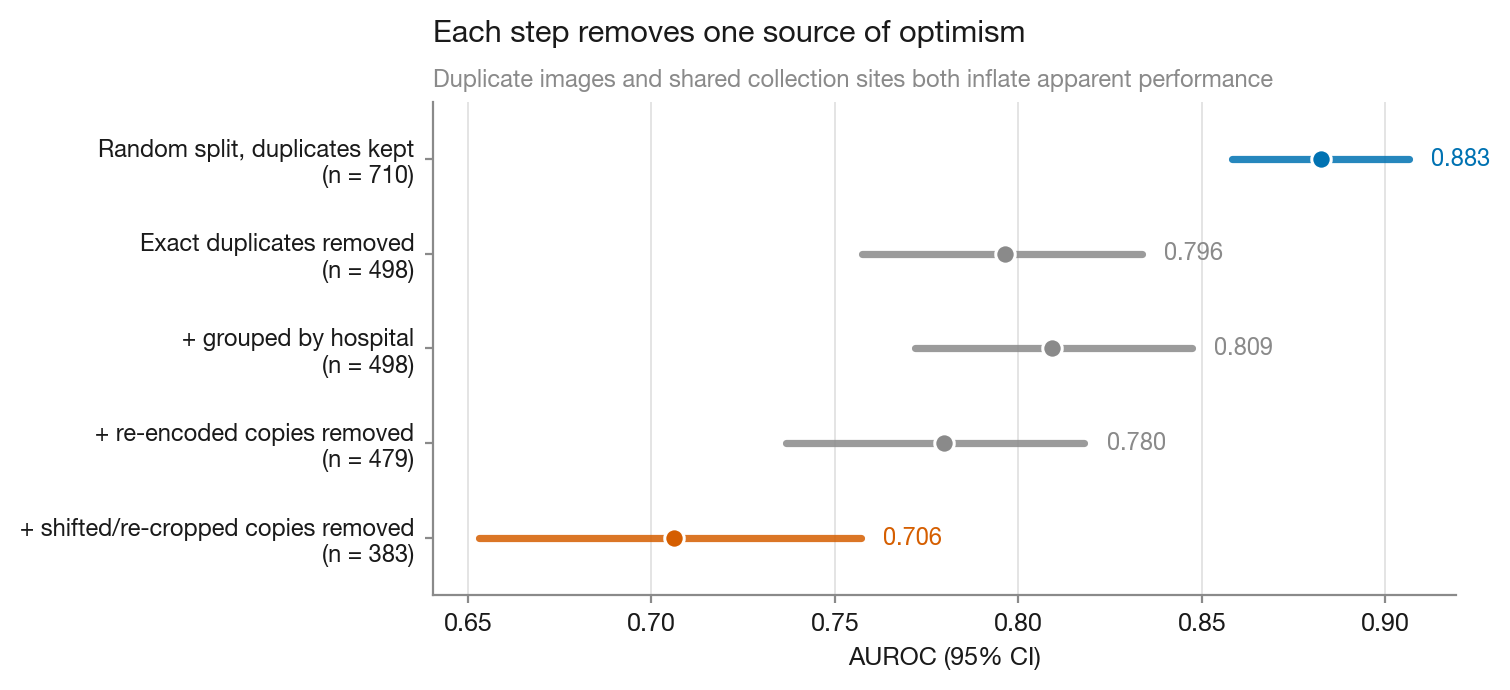
\includegraphics[width=0.78\textwidth]{figs/fig2_leakage.png}
\caption{Apparent performance falls as each source of leakage is removed. The gap between
the first and last bars is the optimism introduced by evaluating on a benchmark whose
records are not distinct.}
\label{fig:leakage}
\end{figure}

\subsection{Does the image contribute?}

A screening score could in principle be driven by demographics alone. Table~\ref{tab:ablation}
rules this out.

\begin{table}[htbp]
\centering
\caption{Feature ablation under the corrected protocol ($n=479$). Comparisons by DeLong's test~\cite{delong1988}.}
\label{tab:ablation}
\small
\begin{tabular}{lcc}
\toprule
Feature set & \auroc{} [95\,\% CI] & vs.\ colour \\
\midrule
Demographics only (age, sex) & 0.565 [0.514--0.618]
  & $\Delta -0.215$, $p=4.4\times10^{-11}$ \\
\textbf{Colour only}         & \textbf{0.780 [0.737--0.818]} & --- \\
Colour + demographics        & 0.769 [0.725--0.808]
  & $\Delta -0.011$, $p=0.30$ \\
\bottomrule
\end{tabular}
\end{table}

The image carries substantial and highly significant signal over demographics. Adding
demographics to colour produces no detectable improvement, which is the expected result if
the photograph already encodes what age and sex would otherwise proxy.
Figure~\ref{fig:roc} shows the corresponding ROC curves.

\begin{figure}[htbp]
\centering
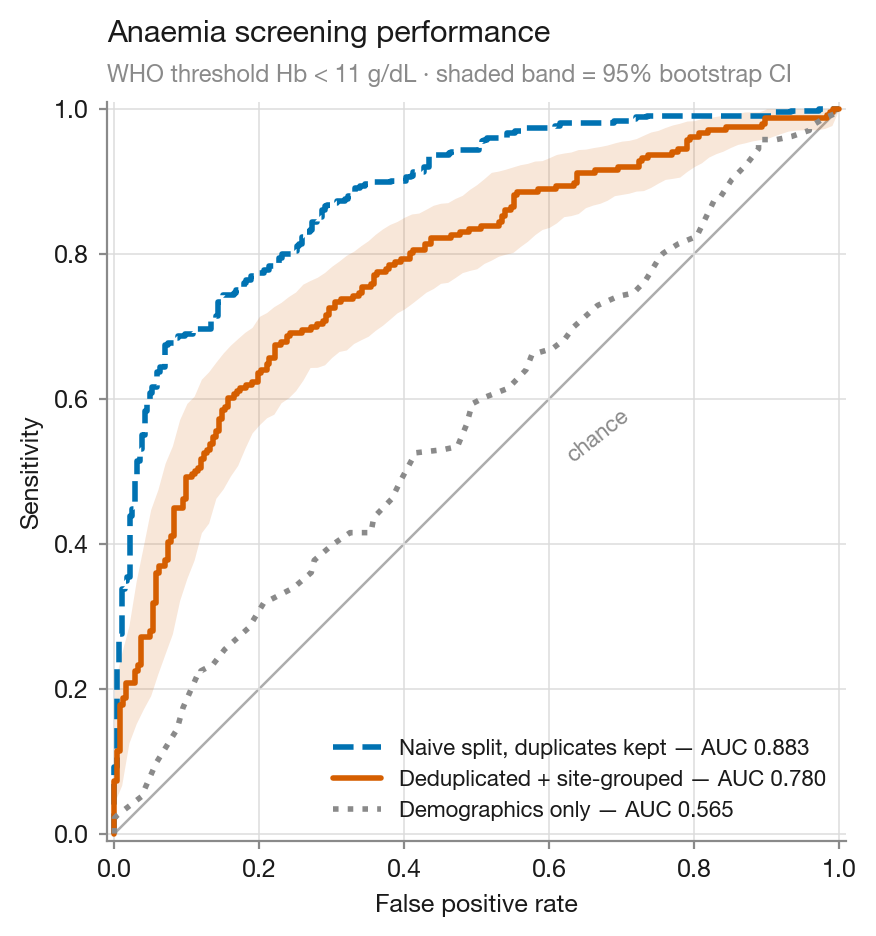
\includegraphics[width=0.68\textwidth]{figs/fig1_roc.png}
\caption{ROC curves under the corrected protocol. Colour features clearly separate from the
demographics-only floor; colour + demographics is indistinguishable from colour alone.}
\label{fig:roc}
\end{figure}

\subsection{Choice of model}

We report both a haemoglobin regressor and a direct binary classifier, because they answer
different questions and we did not wish to adopt the better number after the fact.

\begin{table}[htbp]
\centering
\caption{Regressor versus direct classifier.}
\label{tab:models}
\small
\begin{tabular}{lccc}
\toprule
Model & \auroc{} [95\,\% CI] & Hb output & Agreement assessable \\
\midrule
Hb regressor \emph{(headline)} & 0.780 [0.737--0.818] & yes, MAE 1.46~\gdl & yes \\
Binary classifier              & \textbf{0.818 [0.778--0.854]} & no & no \\
\bottomrule
\end{tabular}
\end{table}

The classifier discriminates better, as expected when the decision is optimised directly,
but it produces no haemoglobin estimate and therefore cannot be examined for clinical
agreement. We retain the regressor as the headline because the agreement result
(Section~\ref{sec:agreement}) is the more consequential finding.

\subsection{Calibration}

\begin{table}[htbp]
\centering
\caption{Post-hoc calibration degrades both calibration and discrimination. Isotonic
calibration applied via \texttt{CalibratedClassifierCV} with $cv=3$.}
\label{tab:calib}
\footnotesize
\begin{tabular}{lccccc}
\toprule
Variant & Brier & ECE & H--L $p$ & \auroc{} & prob.\ range \\
\midrule
\textbf{Uncalibrated} & \textbf{0.174} & \textbf{0.054} & 0.021 & \textbf{0.818} & [0.01, 0.98] \\
Isotonic & 0.200 & 0.116 & $<0.001$ & 0.788 & [0.00, 0.92] \\
\bottomrule
\end{tabular}
\end{table}

Wrapping the model in post-hoc calibration made both calibration and discrimination worse.
The mechanism is visible in the probability range: \texttt{CalibratedClassifierCV} fits $k$
sub-models on $k-1$ folds each and averages them, pulling probabilities toward the centre,
and at roughly 380 training rows each sub-model is additionally data-starved. The result is
systematic \emph{under}-confidence --- the opposite of the over-confidence that calibration is
normally applied to cure. We therefore report the uncalibrated model, which remains slightly
imperfect (Hosmer--Lemeshow $p=0.021$). We note this because the standard recommendation to
calibrate is not unconditional at this sample size.

\begin{figure}[htbp]
\centering
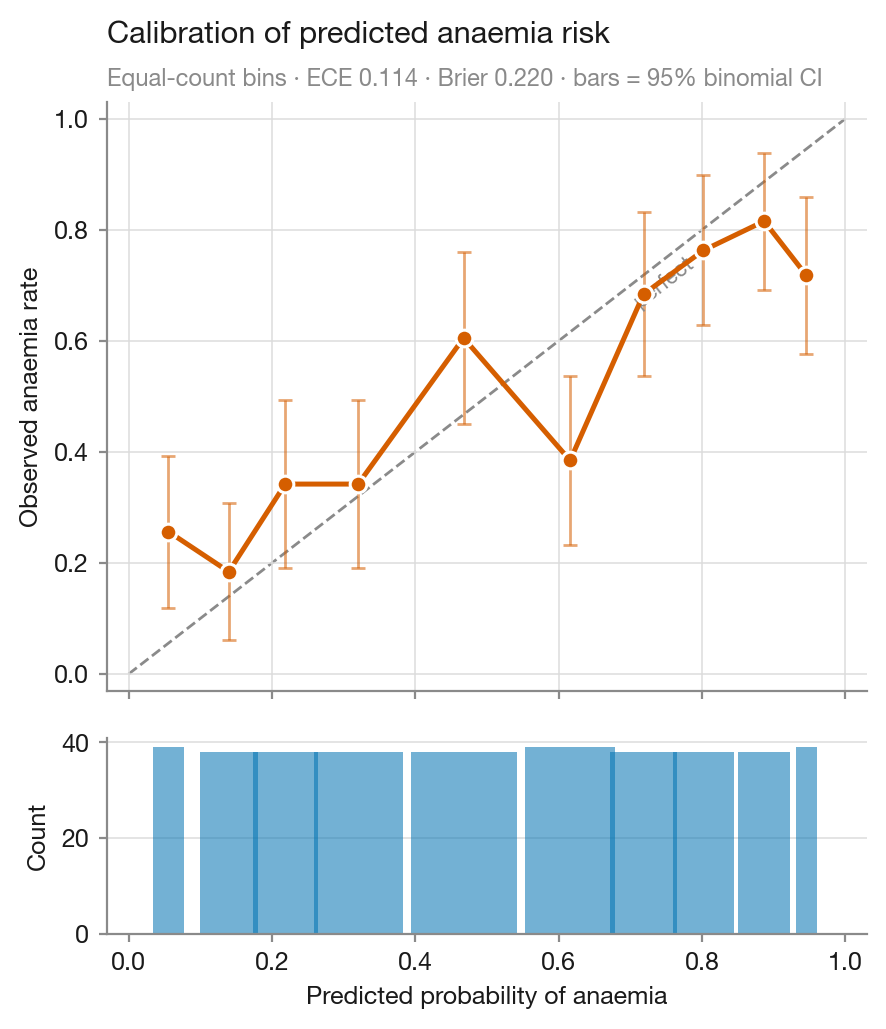
\includegraphics[width=0.68\textwidth]{figs/fig4_calibration.png}
\caption{Reliability curves. Post-hoc isotonic calibration compresses the probability range
and worsens both Brier score and expected calibration error.}
\label{fig:calib}
\end{figure}

\subsection{Screening operating point}

At the WHO threshold the model achieves sensitivity $0.775$ and specificity $0.630$. Tuned
to catch 90\,\% of anaemic children, specificity falls to $0.362$ --- referring roughly
64\,\% of healthy children for confirmatory testing. This, rather than \auroc{}, is the
quantity that determines deployability, and at present it is not good enough for
unsupervised use.

\begin{figure}[htbp]
\centering
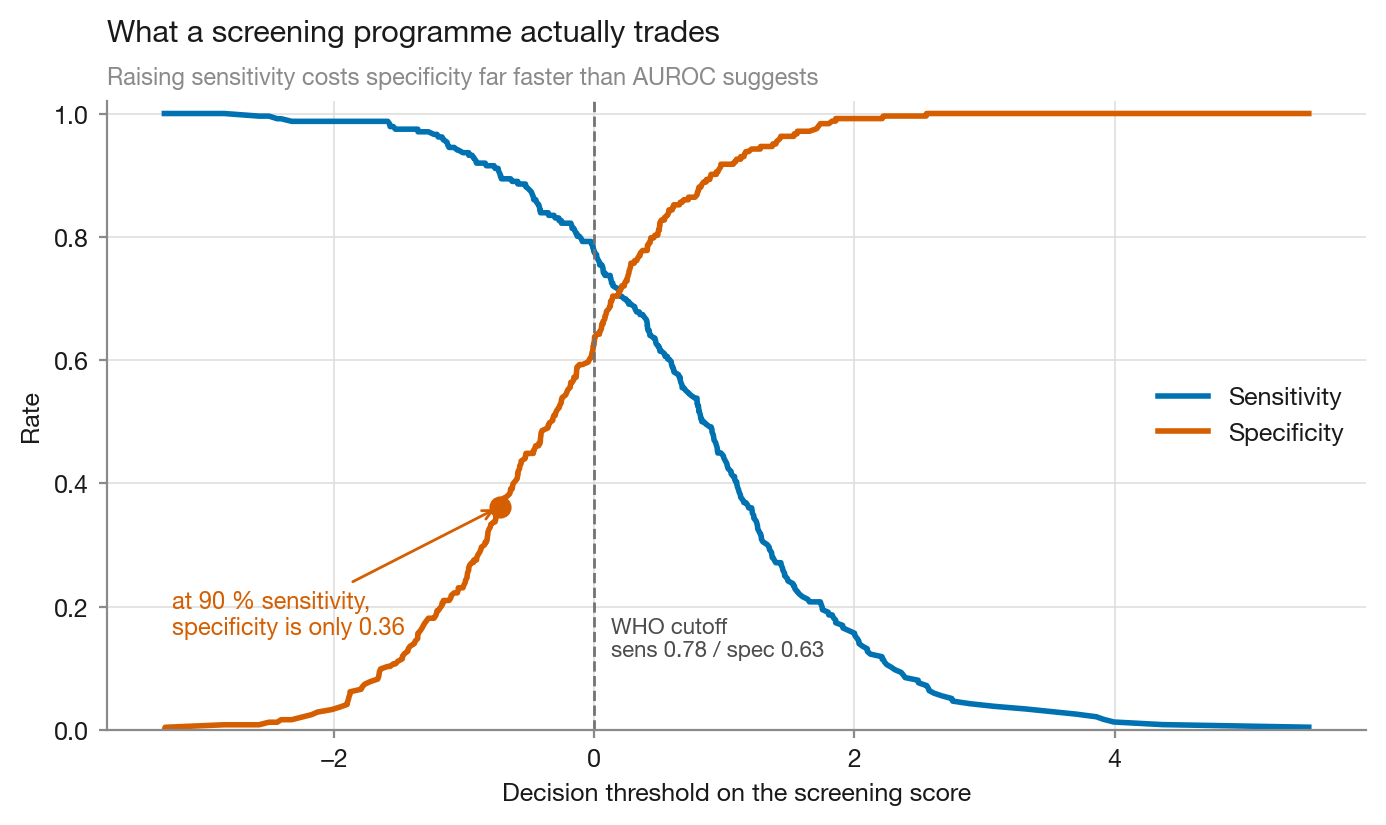
\includegraphics[width=0.82\textwidth]{figs/fig9_operating_point.png}
\caption{Sensitivity and specificity against the decision threshold, from the same out-of-fold
predictions as the headline result. The curves cross steeply: moving from the WHO cutoff to
90\,\% sensitivity costs roughly half the specificity. This trade, rather than \auroc{}, is what a
screening programme has to absorb.}
\label{fig:op}
\end{figure}

\subsection{Agreement as a haemoglobin estimator}
\label{sec:agreement}

Bland--Altman analysis~\cite{blandaltman1986} gives a bias of $+0.03$~\gdl{} with limits of agreement from $-3.65$
to $+3.70$~\gdl, a span of $7.3$~\gdl, and a proportional-bias slope of $-0.67$. The model
shrinks toward the population mean, over-predicting in anaemic children and under-predicting
in healthy ones. A clinically useful non-invasive haemoglobin meter would require limits
nearer $\pm1$~\gdl. \textbf{No haemoglobin value from this model should be reported to a
clinician.}

\begin{figure}[htbp]
\centering
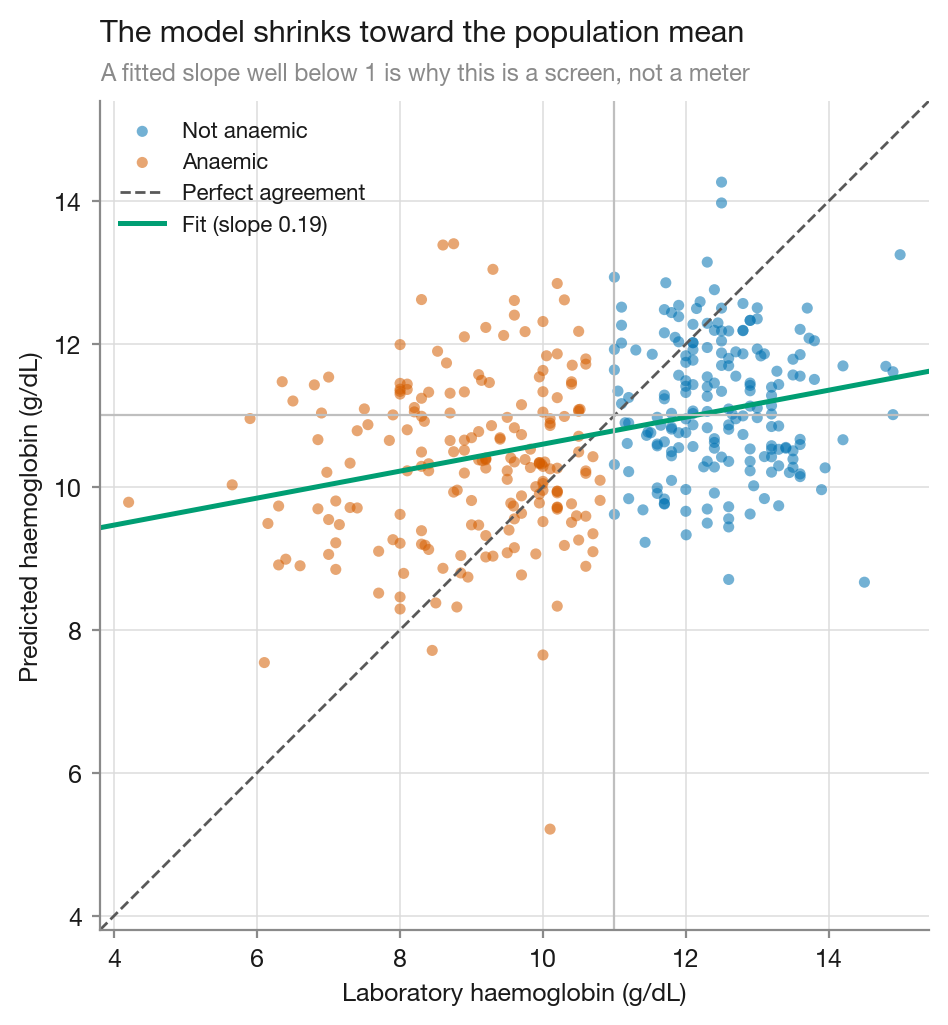
\includegraphics[width=0.60\textwidth]{figs/fig10_pred_vs_actual.png}
\caption{Predicted against laboratory haemoglobin. A least-squares fit through the predictions has
slope $0.28$, far below the identity line: a 1~\gdl{} change in true haemoglobin moves the
prediction by roughly a quarter of that. The model separates anaemic from non-anaemic children
while carrying little information about \emph{how} anaemic they are.}
\label{fig:pva}
\end{figure}

\begin{figure}[htbp]
\centering
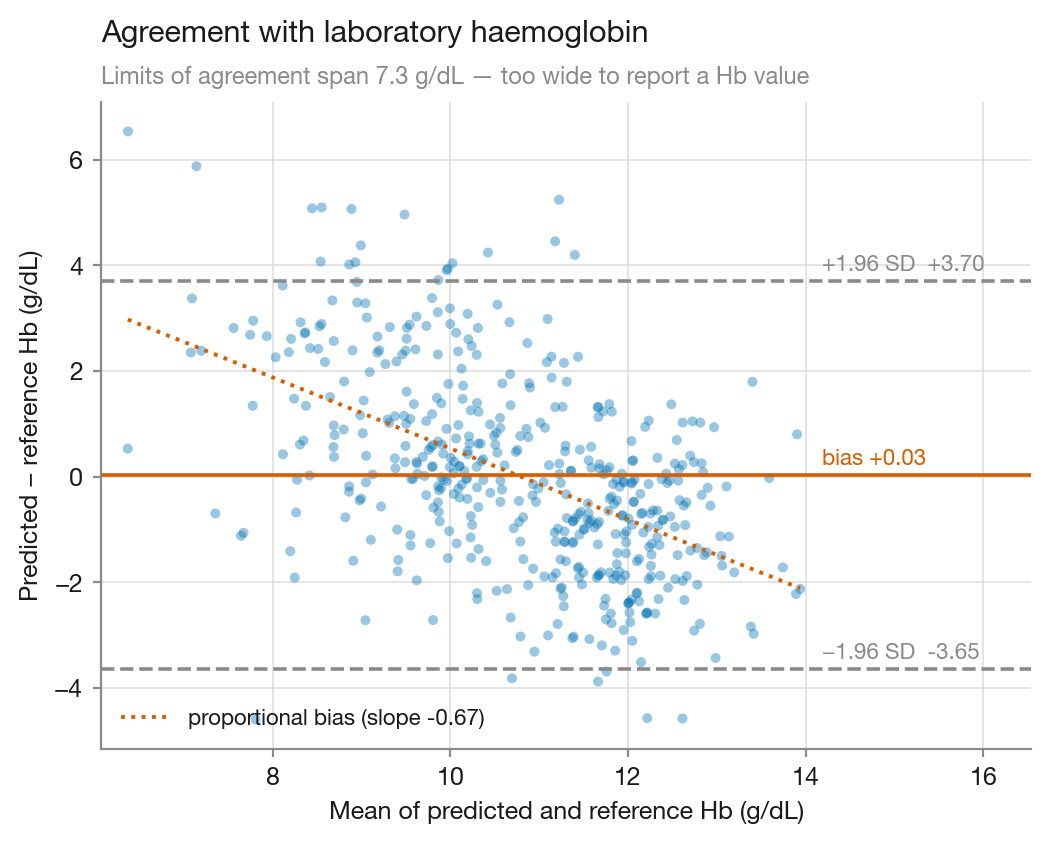
\includegraphics[width=0.68\textwidth]{figs/fig5_bland_altman.png}
\caption{Bland--Altman agreement. The limits span 7.3~\gdl{} and the proportional bias is
pronounced, establishing this as a triage screen rather than a measurement device.}
\label{fig:ba}
\end{figure}

\subsection{Is acting on the model better than the alternatives?}
\label{sec:dca}

Discrimination and calibration describe the model; neither says whether acting on it beats what a
clinic would otherwise do. Where the realistic comparators are ``refer every child'' and ``refer
none'', that comparison is what decides deployment. Decision curve analysis~\cite{vickers2006}
makes it directly, through net benefit

\begin{equation}
\mathrm{NB}(p_t) \;=\; \frac{\mathrm{TP}}{N} \;-\; \frac{\mathrm{FP}}{N}\cdot\frac{p_t}{1-p_t},
\end{equation}

where $p_t$ is the probability at which referral becomes worthwhile and the odds term prices one
missed case against the false referrals a clinic will tolerate for it. A model is worth using only
where its curve lies above both comparators.

Figure~\ref{fig:dca} shows the result, and it is a qualified one. \textbf{Below
$p_t \approx 0.15$ the model is worse than simply referring every child.} That is a direct
consequence of the 49\,\% prevalence in this cohort: when half the children are anaemic and missing
a case is judged far costlier than an unnecessary referral, no triage rule beats referring
everyone. Above that threshold the model does add benefit, and the margin widens as false
referrals become more costly --- at $p_t = 0.4$ its net benefit is $0.29$ against $0.15$ for
referring everyone.

The practical reading is that this model earns its place only where confirmatory testing is scarce
enough that indiscriminate referral is not an option. That is a narrower claim than \auroc{}
$0.780$ suggests on its own, and it is the claim the evidence supports.

\begin{figure}[htbp]
\centering
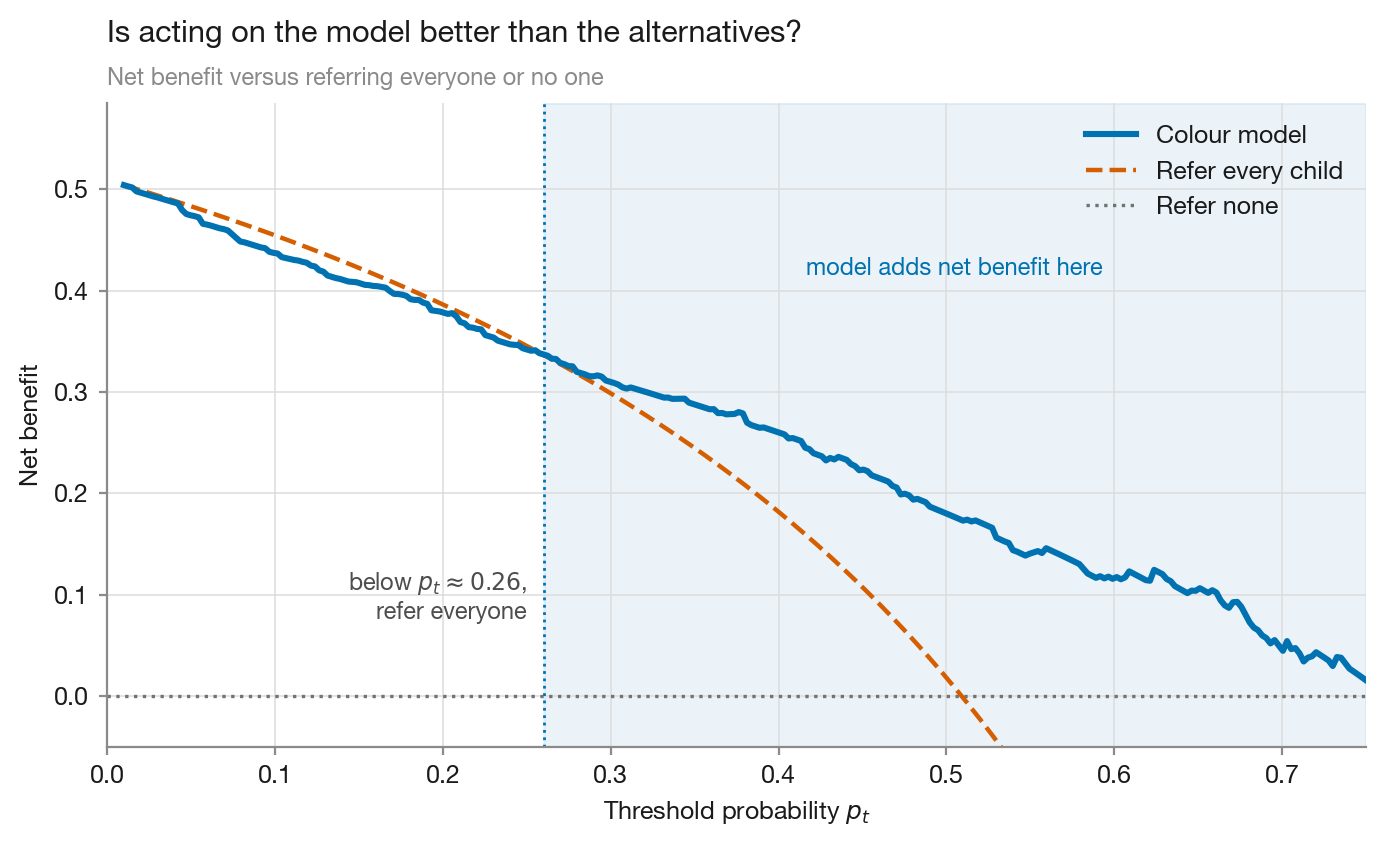
\includegraphics[width=0.82\textwidth]{figs/fig11_decision_curve.png}
\caption{Decision curve analysis. Net benefit of the colour model against the two comparators
available to a clinic. The model is not universally useful: below $p_t \approx 0.15$, referring
every child is the better strategy, a consequence of the high prevalence in this cohort. Its
advantage appears once false referrals carry real cost.}
\label{fig:dca}
\end{figure}

\subsection{Cross-site generalisation}

Leave-one-site-out evaluation across nine evaluable hospitals gives a mean \auroc{} of
$0.820$ (range $0.688$--$1.000$). The perfect score at SDA Hospital arises from $n=11$ at
82\,\% prevalence and should be read as noise rather than performance; the informative
observation is that the \emph{lowest} score belongs to the \emph{largest} site
(Komfo Anokye Teaching Hospital, $n=94$, \auroc{} $0.703$), which is the direction one would
expect if smaller sites are optimistically estimated.

\begin{figure}[htbp]
\centering
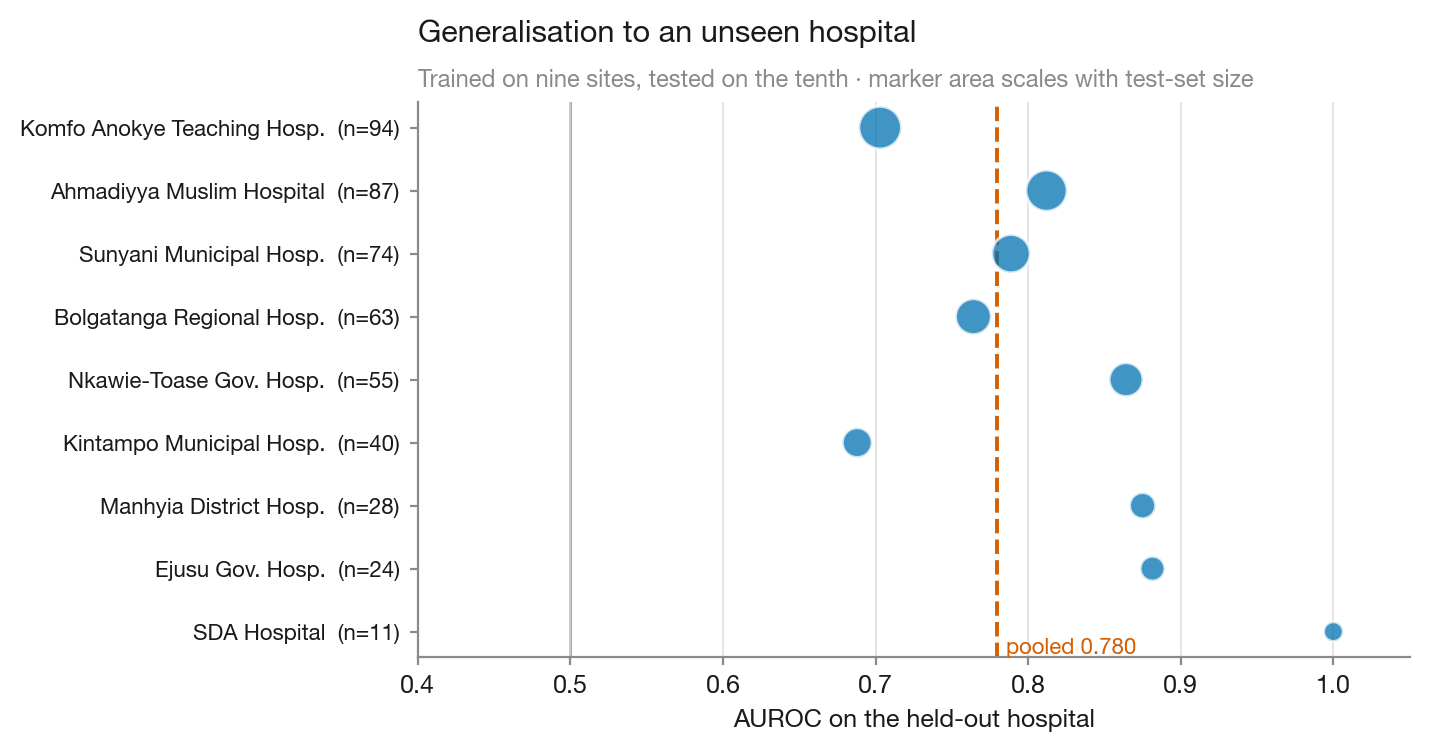
\includegraphics[width=0.72\textwidth]{figs/fig3_sites.png}
\caption{Leave-one-site-out performance. Marker size reflects site $n$; small sites carry
wide, unreliable intervals.}
\label{fig:sites}
\end{figure}

\subsection{Which features carry the signal}

Permutation importance was measured out-of-fold, because the model's internal impurity
importances are computed on training data and are biased toward continuous features.
Saturation ($\Delta$\auroc{} $0.073$) and the 10th percentile of the redness index
($0.055$) dominate, followed by circular mean hue ($0.040$), the redness index ($0.039$) and
mean red ($0.034$). Saturation and the pale tail of the redness distribution are the
physiologically expected carriers of pallor. Because these features are strongly correlated,
a low score should be read as ``redundant given the others'', not ``irrelevant''. Figure~\ref{fig:corr} shows this rather than
assuming it: mean absolute pairwise correlation across the twelve features is $0.51$, reaching
$0.98$ between mean green and CIELAB $L^*$. Two clusters are visible --- an RGB/lightness group and
a saturation-and-redness group --- and permutation importance divides credit within each. That is
why no single feature scores highly even though the set as a whole carries $+0.215$ \auroc{} over
demographics.

\begin{figure}[htbp]
\centering
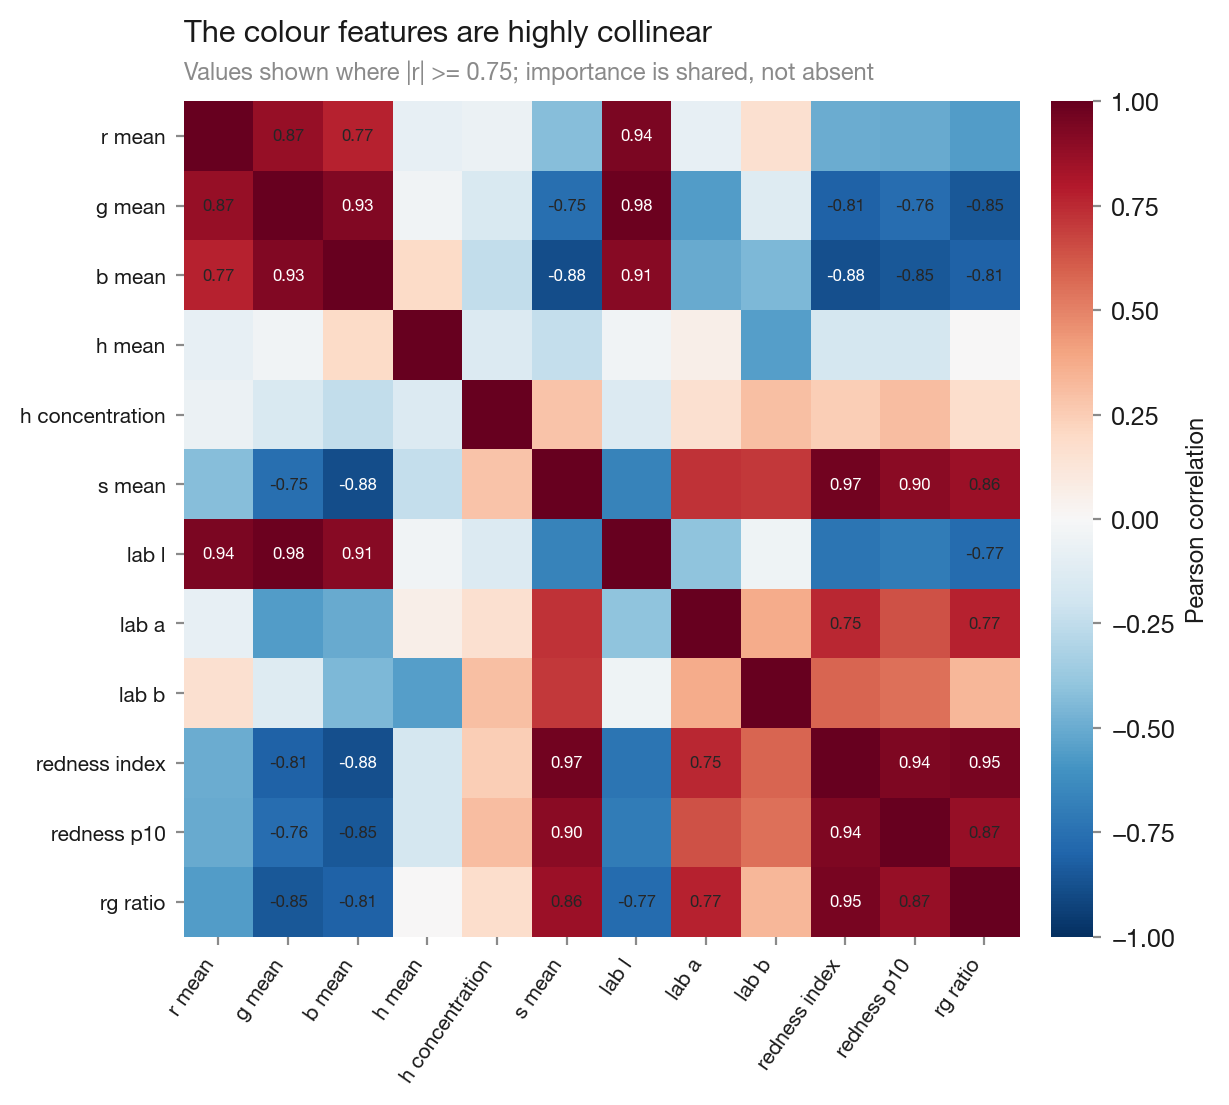
\includegraphics[width=0.70\textwidth]{figs/fig12_feature_correlation.png}
\caption{Pairwise correlation between the twelve colour features, printed where
$|r| \geq 0.75$. This collinearity is why a low permutation-importance score should be read as
redundancy given the rest of the set rather than absence of signal.}
\label{fig:corr}
\end{figure}

\begin{figure}[htbp]
\centering
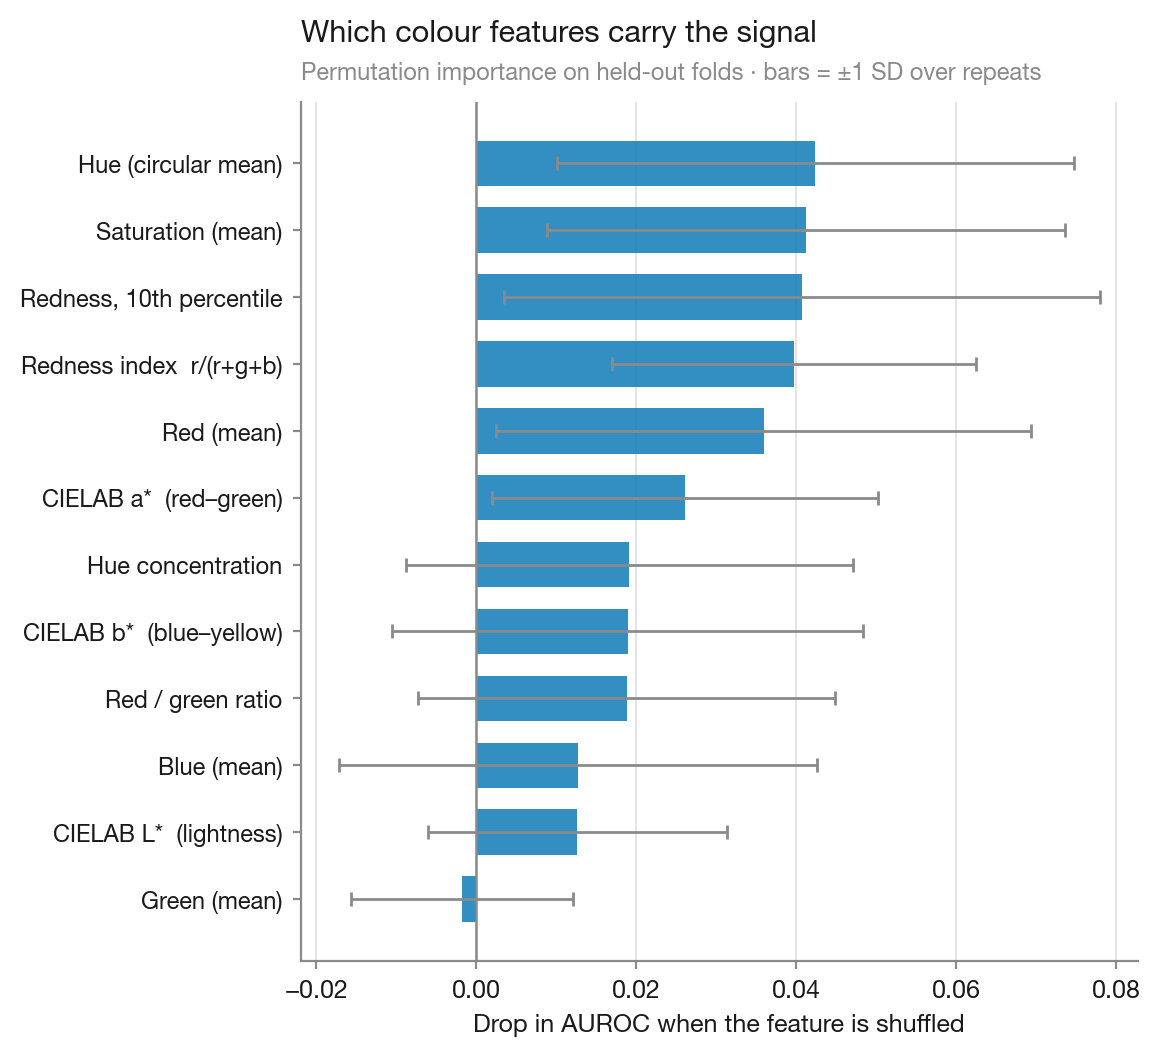
\includegraphics[width=0.68\textwidth]{figs/fig6_importance.png}
\caption{Out-of-fold permutation importance. Saturation and the pale tail of the redness
distribution dominate. Correlated features share credit, so a low score means redundant given the
others rather than uninformative.}
\label{fig:imp}
\end{figure}

\subsection{Controls}
\label{sec:controls}

Table~\ref{tab:controls} lists checks designed to make the headline result fail if it were an
artefact.

\begin{table}[htbp]
\centering
\caption{Adversarial and robustness controls.}
\label{tab:controls}
\footnotesize
\begin{tabular}{lll}
\toprule
Control & Result & Interpretation \\
\midrule
Label permutation (10 repeats)   & \auroc{} $0.507\pm0.026$ & chance; the harness does not leak \\
Seed stability (10 seeds)        & $0.778\pm0.003$          & not fold-assignment luck \\
Bootstrap vs.\ DeLong CI         & [0.737, 0.818] vs.\ [0.738, 0.821] & independent machinery agrees \\
Unambiguous singles only ($n=407$) & 0.763                  & holds where no label conflict exists \\
Nested-CV hyperparameter tuning  & $0.780 \to 0.782$        & fixed settings not cherry-picked \\
Duplicate-threshold sweep (0.5--5.0) & 0.774--0.784         & conclusion not sensitive to cutoff \\
\bottomrule
\end{tabular}
\end{table}

\begin{figure}[htbp]
\centering
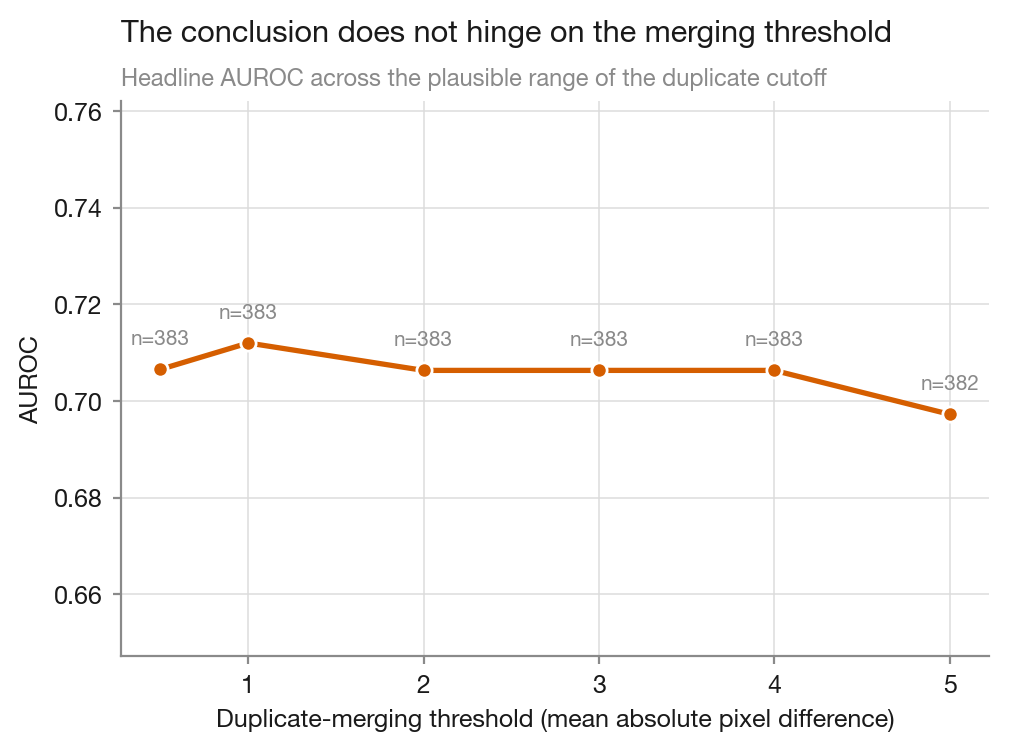
\includegraphics[width=0.66\textwidth]{figs/fig8_threshold.png}
\caption{Sensitivity of the headline result to the perceptual duplicate-detection threshold.
AUROC varies between 0.774 and 0.784 across the sweep, so the conclusion does not depend on where
the cutoff is placed.}
\label{fig:thr}
\end{figure}

\subsection{Would more data help?}

A learning curve over training-set size rises from \auroc{} $0.635$ at 120 images to $0.782$
at 479 and is still climbing at full size. Performance here is therefore limited by sample
size as well as by the dataset's irreducible label noise; a larger, cleanly labelled dataset
would plausibly exceed $0.780$.

\begin{figure}[htbp]
\centering
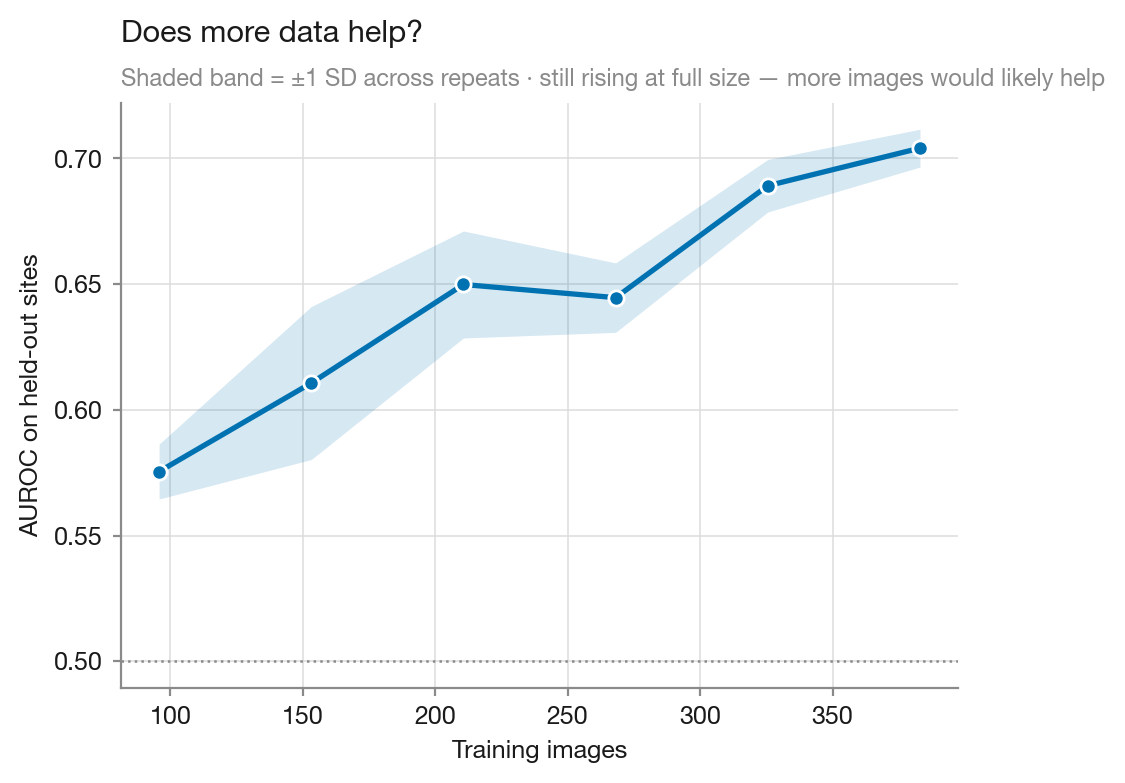
\includegraphics[width=0.66\textwidth]{figs/fig7_learning_curve.png}
\caption{Learning curve. The absence of a plateau indicates the benchmark is sample-limited.}
\label{fig:lc}
\end{figure}

\section{Discussion}

The gap between $0.883$ and $0.780$ is not a modelling result; it is an artefact of dataset
handling. It matters because it is the kind of gap that separates a method reported as
promising from one reported as marginal, and because nothing about the naive protocol looks
careless from the inside --- a random split is the default, and duplicates are invisible
unless specifically sought. The 19 images that are pixel-identical only after
region-of-interest extraction are a particularly awkward case: a reasonable practitioner who
deduplicates by file hash would still be leaking.

Our corrected baseline should be read as establishing a floor for interpretable colour
features, not a ceiling for the task. Learned representations may well exceed it. The
purpose of reporting it is that any such claim can now be measured against a number produced
under controls that are stated and reproducible.

The clinical framing deserves emphasis. Discrimination at \auroc{} $0.780$ is not
uninteresting for triage in a setting where the alternative is no screening at all. But the
Bland--Altman result forecloses use as a haemoglobin estimator, and the operating point ---
64\,\% of healthy children referred at 90\,\% sensitivity --- would impose a confirmatory
testing burden that may exceed what a low-resource clinic can absorb. Both numbers are more
decision-relevant than the \auroc{} that such studies typically headline.

\section{Limitations}

\begin{itemize}
  \item \textbf{Label noise is irreducible.} Ninety duplicate groups carry conflicting
        haemoglobin on identical pixels; median merging cannot recover the truth, and a
        performance ceiling is therefore built into the benchmark.
  \item \textbf{No colour calibration.} No colour card or white-balance reference was
        captured, so absolute RGB partly encodes illumination. Normalised ratios mitigate
        but do not eliminate this.
  \item \textbf{One country, one age band.} Children 6--59 months in Ghana. Nothing here
        supports use in adults, in pregnancy, or across different skin tones and camera
        pipelines.
  \item \textbf{Hand-drawn masks.} A deployed system would require automatic conjunctiva
        segmentation, whose error is not represented in any number reported here.
  \item \textbf{No true external validation.} Leave-one-site-out varies camera, operator and
        prevalence, but not country or protocol. Validation on an independent dataset is the
        obvious next step.
  \item \textbf{Not a clinical device.} No regulatory, ethical or safety assessment has been
        performed. This is a software study on a public dataset.
\end{itemize}

\section{Conclusion}

CP-AnemiC contains duplicate records --- including duplicates that survive content hashing
and duplicates carrying conflicting labels --- at a scale that inflates \auroc{} by
approximately $0.10$ under a random split. We recommend that future work on this benchmark
deduplicate at the pixel level within the annotated region and group cross-validation folds
by collection site.

Under those controls, twelve interpretable colour features achieve \auroc{}
$0.780$ (95\,\% CI $0.737$--$0.818$) for WHO childhood anaemia, with the image contributing
$+0.215$ over demographics alone. The resulting model is a plausible triage screen and is
not a haemoglobin meter: limits of agreement span $7.3$~\gdl{} and specificity falls to
$0.362$ at 90\,\% sensitivity. Reporting these quantities alongside \auroc{} is, we suggest,
the minimum needed to judge whether such a method could be deployed.

\section*{Acknowledgements}

% ACTION REQUIRED: add anyone who helped -- supervisors, endorsers, anyone who
% read a draft. Delete this comment before submitting.

\section*{Use of generative AI}

Generative AI (Anthropic Claude) was used to draft and typeset this manuscript from the
author's own analysis, results and written findings, and to assist with the accompanying
analysis code. The study design, the dataset audit and duplicate-leakage discovery, the
choice of controls, and the interpretation of results are the author's own. The author has
reviewed and verified the entire manuscript, including every reported figure, and takes full
responsibility for its content.

\section*{Reproducibility}

The complete analysis runs in approximately 80~seconds on a laptop:

\begin{quote}\ttfamily\small
pip install -r requirements.txt\\
\# download CP-AnemiC into data/cp-anemic/\\
python3 scripts/run\_full\_analysis.py\\
python3 -m pytest tests/ -q
\end{quote}

Every number and figure in this paper is regenerated by that script. The accompanying test
suite (62 tests) is organised by failure mode --- split integrity, feature correctness,
numerical robustness, determinism, statistical machinery, and adversarial nulls --- on the
principle that the dangerous failure in this setting is not a crash but a plausible wrong
number.

\section*{Data availability}

CP-AnemiC is publicly available from Mendeley Data
(\href{https://data.mendeley.com/datasets/m53vz6b7fx/1}{\texttt{m53vz6b7fx}})
\cite{asare2023cpanemic} and is used under its published licence. No patient-identifiable
data is redistributed. Derived colour statistics only are stored in the accompanying
repository.

\section*{Conflicts of interest}

None declared.

\begin{thebibliography}{9}

\bibitem{asare2023cpanemic}
J.~W. Asare, P.~Appiahene, and E.~T. Donkoh,
\newblock ``CP-AnemiC: A conjunctival pallor dataset and benchmark for anemia detection in
children,''
\newblock \emph{Mendeley Data}, \texttt{m53vz6b7fx}, 2023.

\bibitem{stevens2022}
G.~A. Stevens, C.~J. Paciorek, M.~C. Flores-Urrutia, et al.,
\newblock ``National, regional, and global estimates of anaemia by severity in women and children
for 2000--19: a pooled analysis of population-representative data,''
\newblock \emph{The Lancet Global Health}, vol.~10, no.~5, pp.~e627--e639, 2022.

\bibitem{who2011}
World Health Organization,
\newblock ``Haemoglobin concentrations for the diagnosis of anaemia and assessment of
severity,''
\newblock \emph{Vitamin and Mineral Nutrition Information System}, WHO/NMH/NHD/MNM/11.1,
Geneva, 2011.

\bibitem{vickers2006}
A.~J. Vickers and E.~B. Elkin,
\newblock ``Decision curve analysis: a novel method for evaluating prediction models,''
\newblock \emph{Medical Decision Making}, vol.~26, no.~6, pp.~565--574, 2006.

\bibitem{delong1988}
E.~R. DeLong, D.~M. DeLong, and D.~L. Clarke-Pearson,
\newblock ``Comparing the areas under two or more correlated receiver operating
characteristic curves: a nonparametric approach,''
\newblock \emph{Biometrics}, vol.~44, no.~3, pp.~837--845, 1988.

\bibitem{blandaltman1986}
J.~M. Bland and D.~G. Altman,
\newblock ``Statistical methods for assessing agreement between two methods of clinical
measurement,''
\newblock \emph{The Lancet}, vol.~327, no.~8476, pp.~307--310, 1986.

\end{thebibliography}

\end{document}
